\chapter{Previous work}
\label{ch:previous_work}

As mentioned in the problem statement in \cref{sec:problem} the focus of the implementations underlying this thesis is to develop multiple strategies to extract a triangulated surface mesh from the data model used inside the VML.
To ease the understanding of the implementations presented in this thesis, a short introduction to the VML and its data model is given.
Parts of this description have been taken from the author's bachelor thesis, where the data model has been previously described with a focus on visualization \cite{bachelor}.

\section{Project history}
\label{sec:project_history}

% TODO: rethink choice of past vs. present tense
From the middle of 2011 to the end of 2013 the project Enlight was conducted for research by the RISC Software GmbH in Hagenberg im Mühlkreis, Austria.
Enlight's goals were the development of a faster, scalable and numerically stable method for modeling and visualizing subtractive manufacturing.
Enlight uses a regular grid data structure to store a stock solid and add precomputed swept volumes.
A triangle elimination strategy is employed to keep the total number of triangles held by the grid within manageable bounds, \cf classification in \cref{sec:classification}.
For visualization, a custom raycasting approach was developed \cite{enlight} and accelerated using GPUs and many-core architectures.

From the beginning to the end of 2014, the follow-up research project Engrave focused on solving swept volume computation for arbitrary cutter geometries and tool paths.
Engrave basically allows dynamic swept volume computation from a set of cutter solids and transformation lists.
Swept volume computation is done by extruding a point cloud along the tool path and then reconstructing a closed triangle mesh from it using a parallel and highly optimized variant of the ball pivoting algorithm \cite{engrave}.
The computed swept volumes where directly imported into Enlight's data model.

With the beginning of 2015, the prototype developed during Enlight and Engrave was rebranded to Virtual Machining Library (VML) and, later that year, to Virtual Modeling Library.
The VML is currently further developed as a commercial product.
\Cref{fig:vml_demo} shows a small demonstration of the VML.

\begin{figure}[h]
	\centering
		\begin{subfigure}[t]{0.32\textwidth}
			\centering
			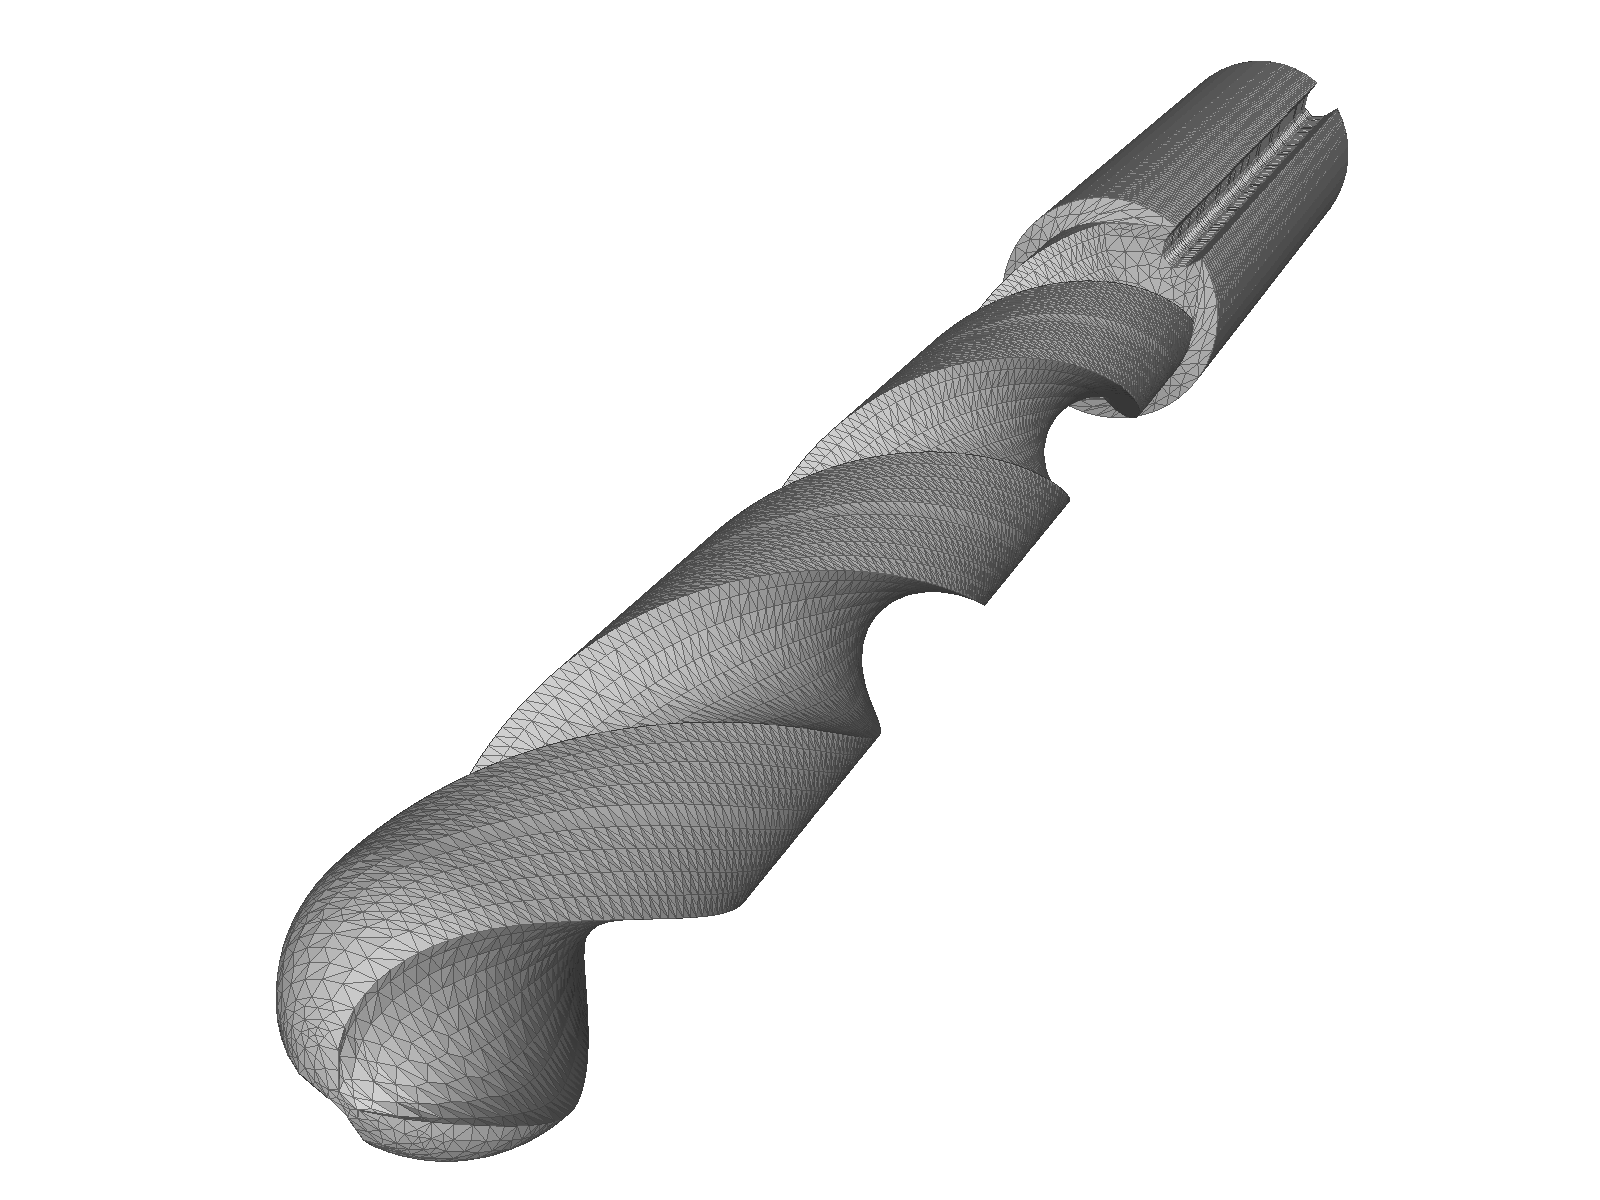
\includegraphics[width=\textwidth]{images/hq_impeller_tool}
			\caption{Ball-end cutter.}
			\label{fig:hq_impeller_tool}
		\end{subfigure}
		\begin{subfigure}[t]{0.32\textwidth}
			\centering
			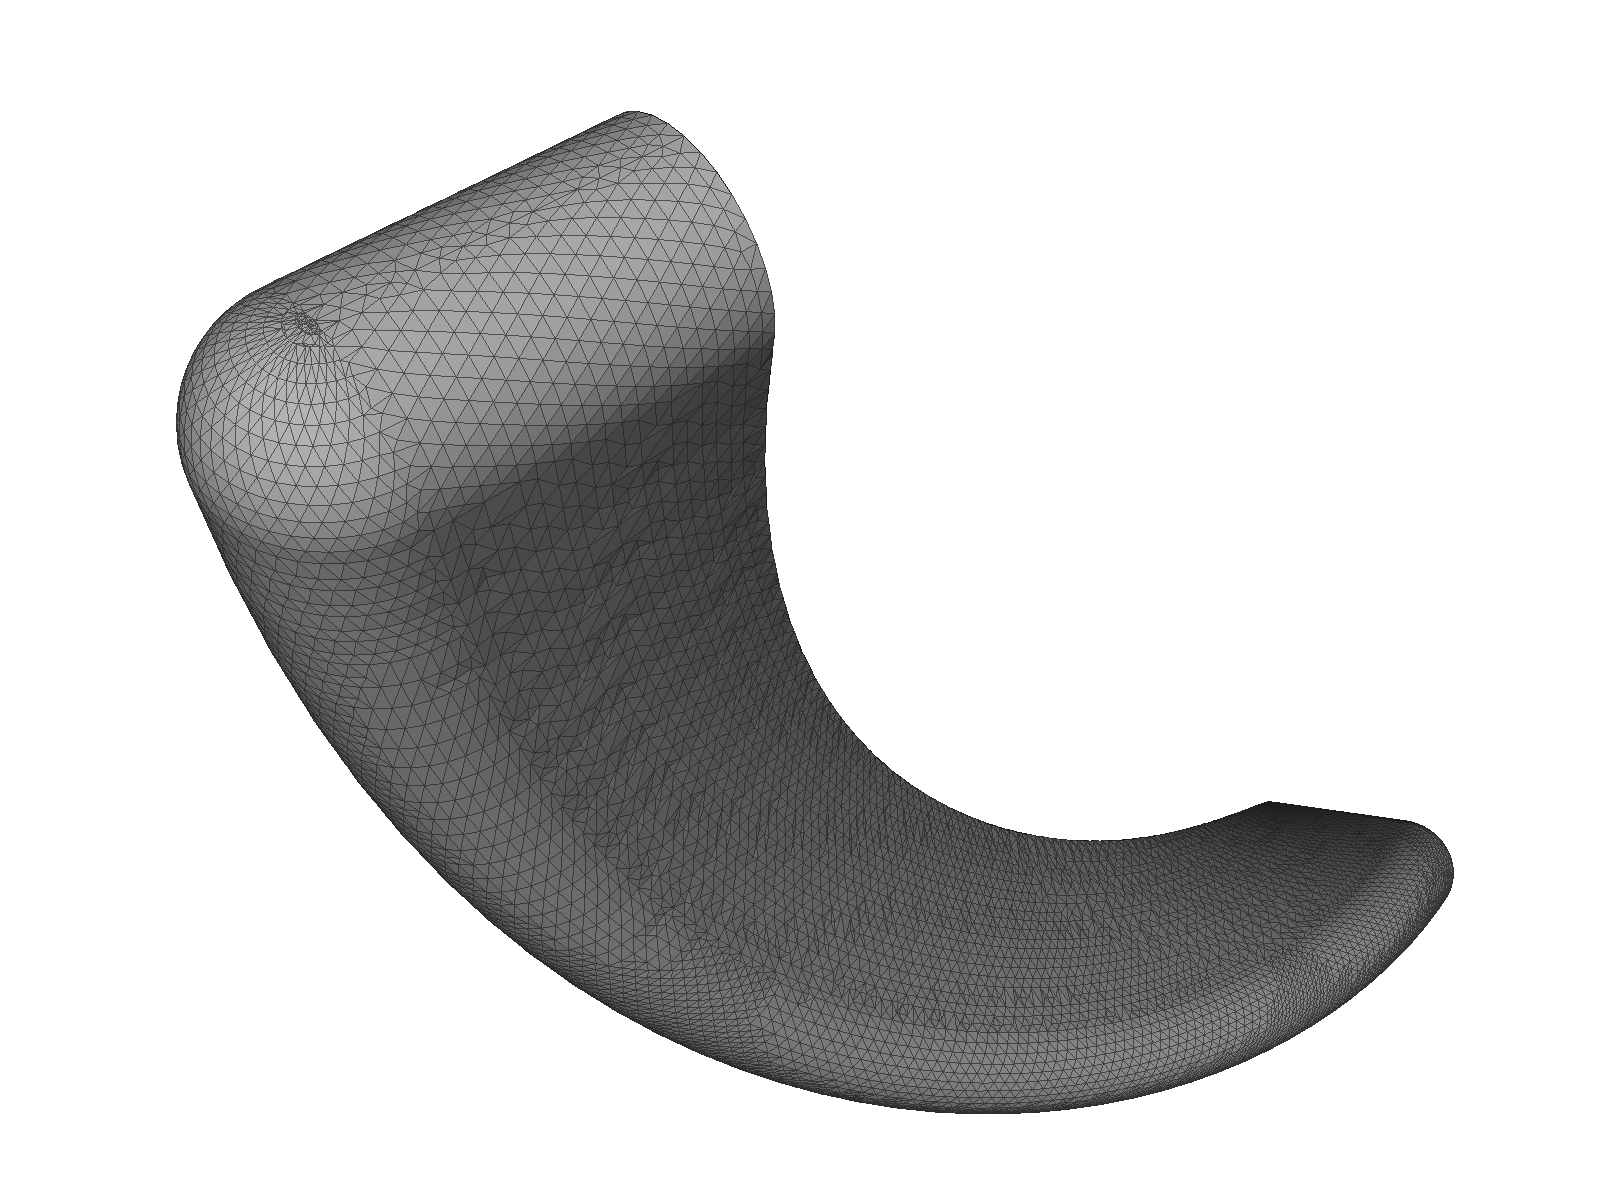
\includegraphics[width=\textwidth]{images/hq_impeller_swept}
			\caption{Swept volume.}
			\label{fig:hq_impeller_swept}
		\end{subfigure}
		\begin{subfigure}[t]{0.32\textwidth}
			\centering
			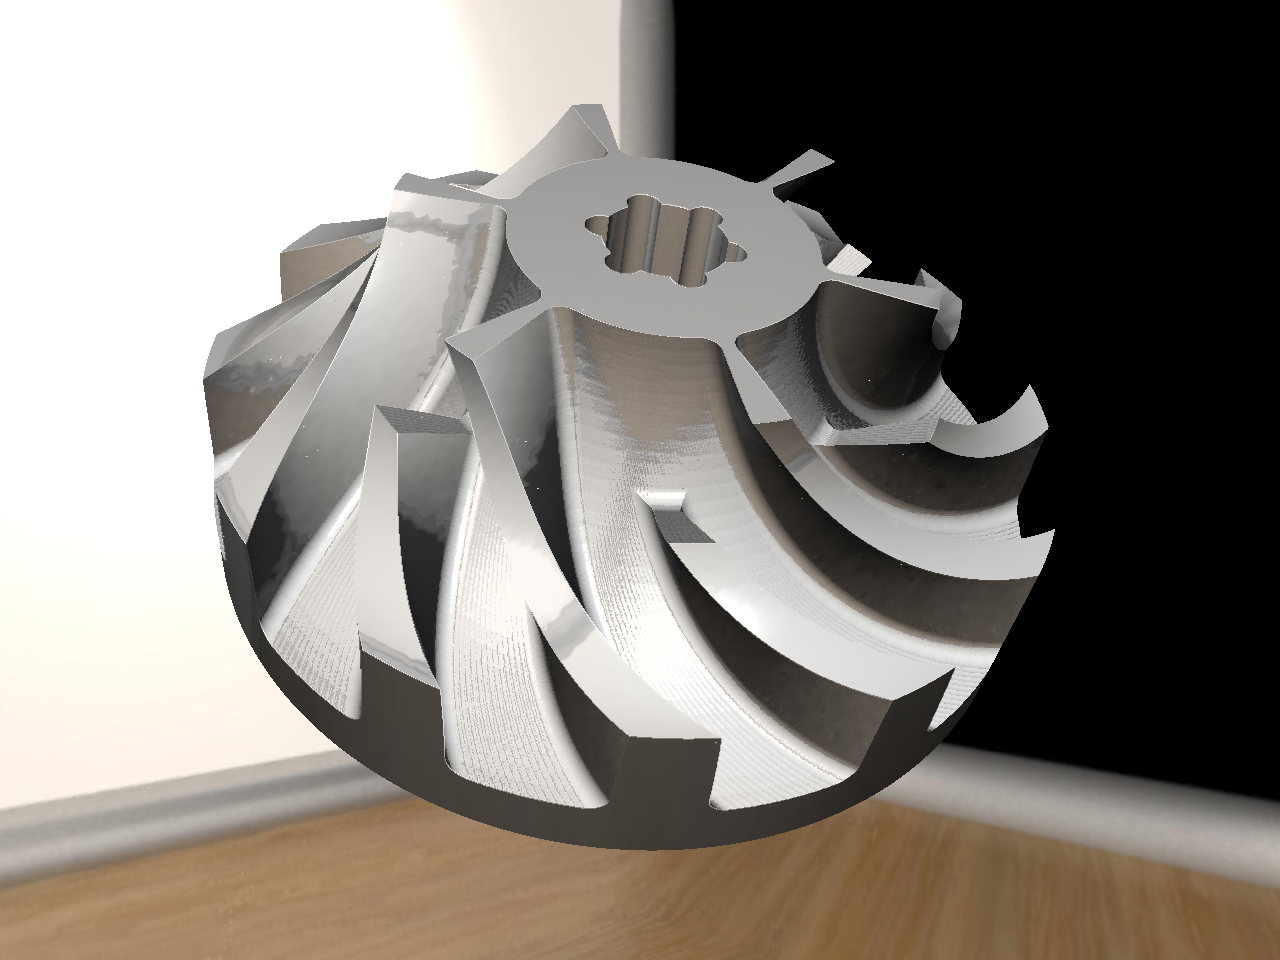
\includegraphics[width=\textwidth]{images/hq_impeller_complete}
			\caption{Machined impeller.}
			\label{fig:hq_impeller_complete}
		\end{subfigure}
		\\
		\begin{subfigure}[t]{0.32\textwidth}
			\centering
			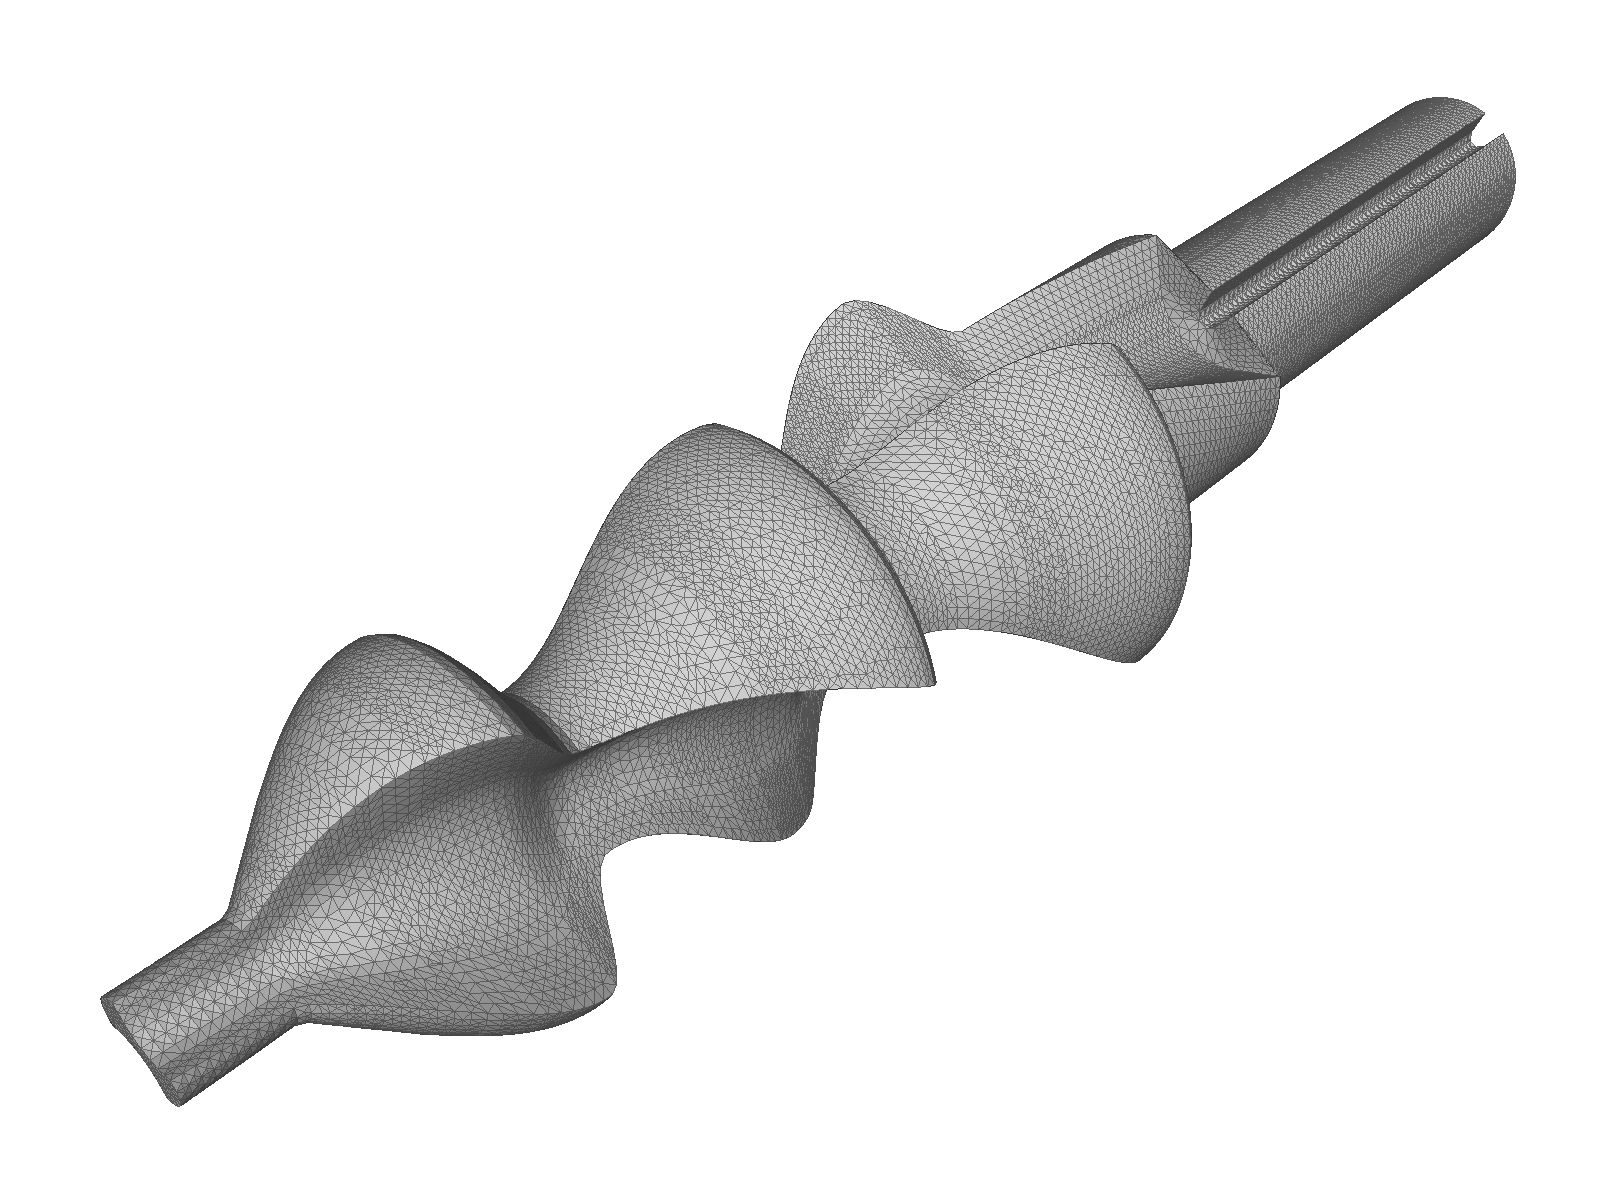
\includegraphics[width=\textwidth]{images/turbine_tool}
			\caption{Fir tree cutter.}
			\label{fig:turbine_tool}
		\end{subfigure}
		\begin{subfigure}[t]{0.32\textwidth}
			\centering
			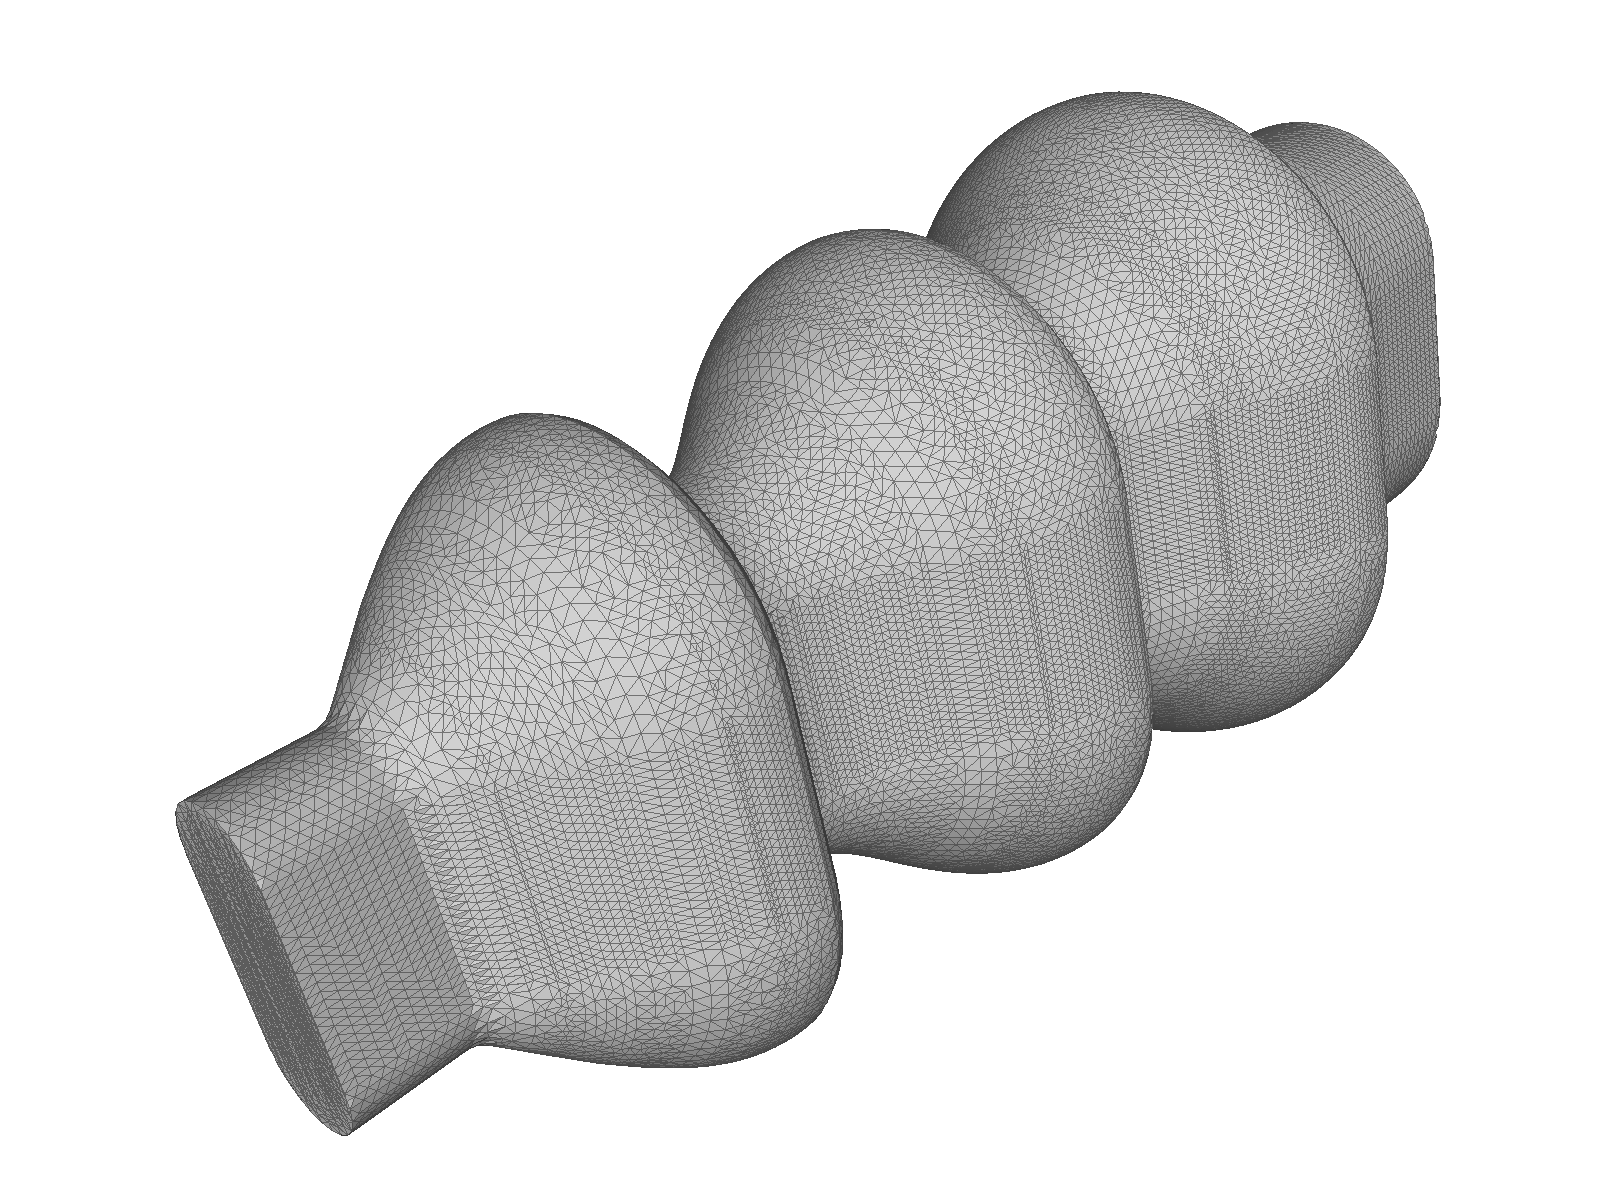
\includegraphics[width=\textwidth]{images/turbine_swept}
			\caption{Swept volume.}
			\label{fig:turbine_swept}
		\end{subfigure}
		\begin{subfigure}[t]{0.32\textwidth}
			\centering
			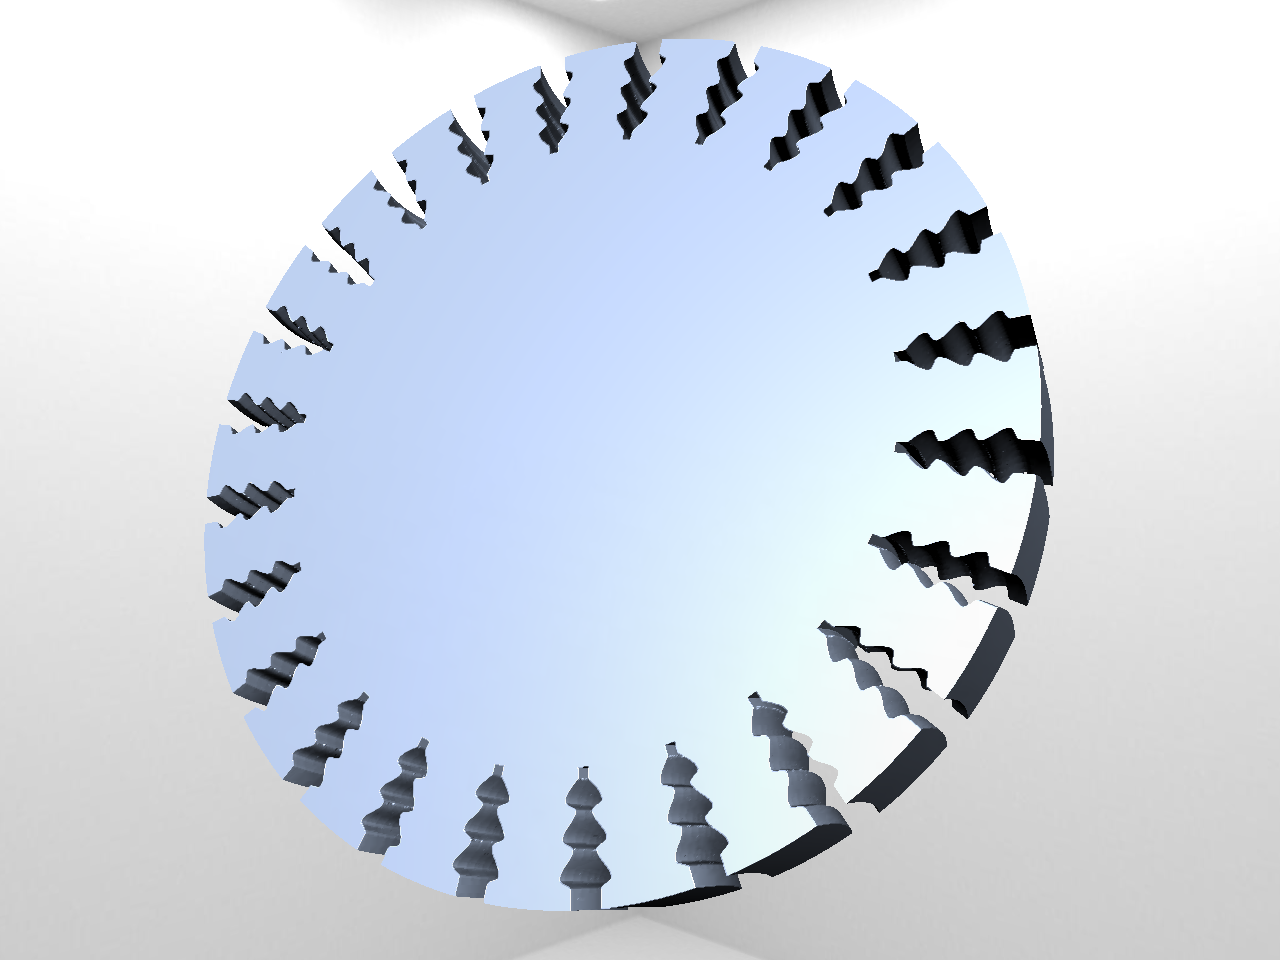
\includegraphics[width=\textwidth]{images/turbine_complete}
			\caption{Machined turbine wheel.}
			\label{fig:turbine_complete}
		\end{subfigure}
	\caption[VML demo]{
		Demonstration of the VML's capabilities.
		Cutter meshes, \cf \subref{fig:hq_impeller_tool} and~\subref{fig:turbine_tool}, are loaded and then transformed using a list of transformation matrices to calculate swept volumes, \cf \subref{fig:hq_impeller_swept} and~\subref{fig:turbine_swept}.
		By applying a series of these swept volumes to a stock, the machining of a workpiece is simulated.
		The result can be visualized using raycasting, \cf \subref{fig:hq_impeller_complete} and~\subref{fig:turbine_complete} \cite{engrave_report}.
	}
	\label{fig:vml_demo}
\end{figure}


\section{VML data model}
\label{sec:vml_data_model}

The primary purpose of the VML is to model, simulate and visualize subtractive manufacturing.
A typical workflow consists of loading a stock solid and then repeatedly sweeping various cutting tools over the stock.
These cutting tools are solid triangle meshes, loaded from disk, which are moved along paths, \ie lists of transformation matrices, to create swept volumes, \ie triangle meshes.
These swept volumes are then conceptually subtracted from the stock.
In fact, swept volumes are stored side by side together with the stock and theoretically build up a specialized CSG tree as shown in \cref{fig:vml_csg}.
A separate processing step is required to calculate the exact surface.
For visualization, the data model is sampled using a raycast which calculates a point on the surface for each ray, \cf \cref{sec:raycasting}.

\begin{figure}[h]
	\centering
	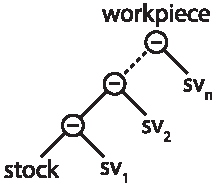
\includegraphics[width=0.5\textwidth]{images/vml_csg}
	\caption[VML CSG representation]{
		The input model held by the VML is similar to a linearized CSG tree.
		The initial stock solid is combined with a series of swept volumes using Boolean subtraction.
		The VML stores parts of the geometries of all leaves of this tree, \cf classification in \cref{sec:classification}.
	}
	\label{fig:vml_csg}
\end{figure}


The central data structure inside the VML, which holds the current state of the simulation, \ie the workpiece, is a regular 3-dimensional grid.
This data structure was originally chosen because it was directly used as acceleration structure for the raycasting subsystem.
Although there is a wide variety of acceleration structures available, \eg kd-trees, octrees, binary space partitioning (BSP) or bounding volume hierarchies (BVH), regular grids offer greater simplicity in organization and construction than the others.
This is especially beneficial in cases where those data structures have to be updated regularly.
Particularly animated scenes in computer-animated films or changing geometries as in virtual machining require frequent rebuilds or updates of those data structures.
Due to their simplicity and regularity, regular grids provide viable candidates for these scenarios.
However, the VML's regular grid is also the basis for a triangle count optimization called classification which is described in the following section.


\subsection{Classification}
\label{sec:classification}

Every time a solid triangle mesh, stock or swept volume, is added to the grid, the triangles of the mesh have to be mapped to the cells of the grid.
Thereby, each triangle is added to each cell it intersects.
A triangle is therefore potentially referenced from multiple cells.
When the mapping is complete, the affected cells are classified into one of three categories with respect to the newly added mesh.
Cells which are occupied by triangles of the mesh's surface are surface cells.
Cells inside and outside the mesh are inside and outside cells and contain no triangles.
The sketches in \cref{fig:classification_before,fig:classification_sv} illustrate the classification of a single solid inside the grid, \ie stock, as well as a swept volume before it is merged.

\begin{figure}[!h]
	\centering
	\begin{tabular}{cc}
		\begin{subfigure}[t]{0.3\textwidth}
			\centering
			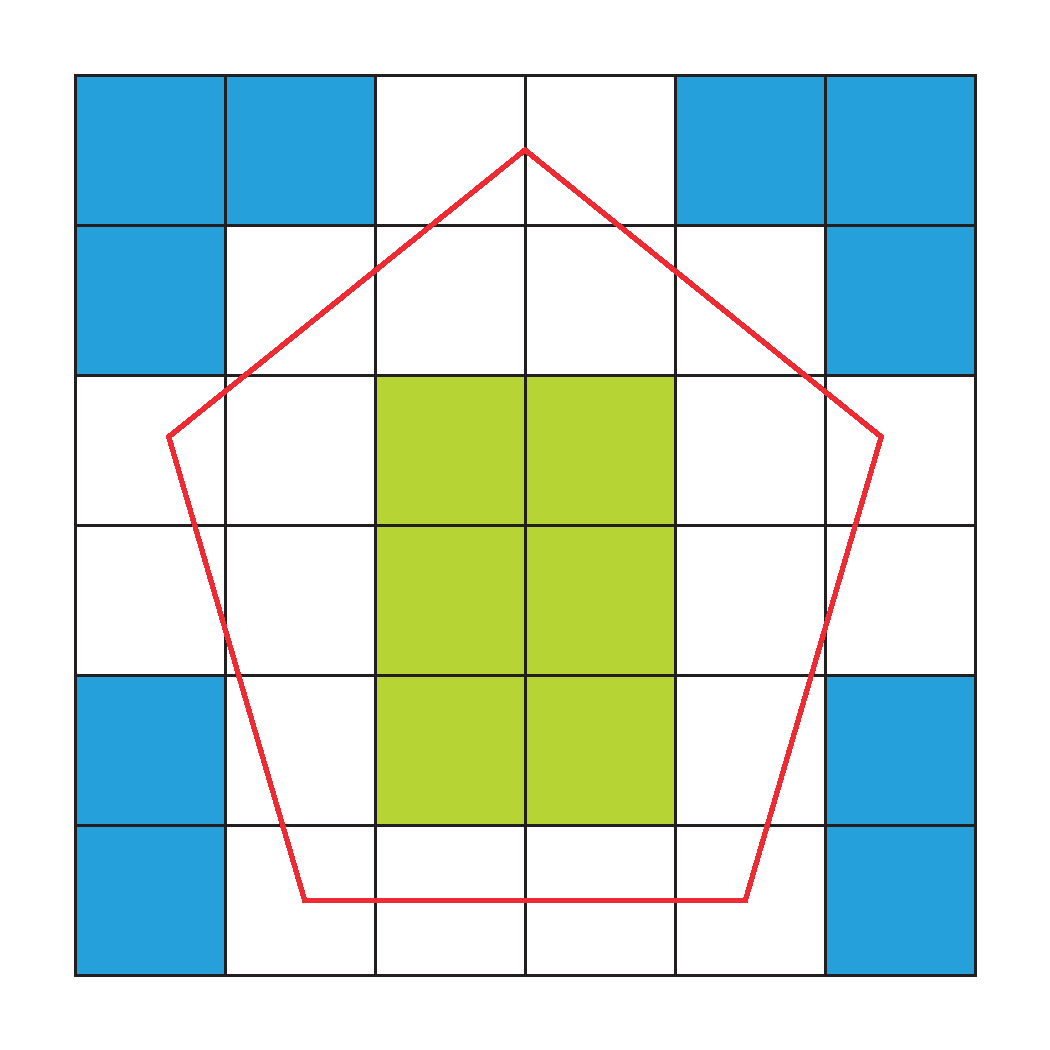
\includegraphics[width=\textwidth]{images/classification_before}
			\caption{Stock}
			\label{fig:classification_before}
		\end{subfigure}&
		\begin{subfigure}[t]{0.3\textwidth}
			\centering
			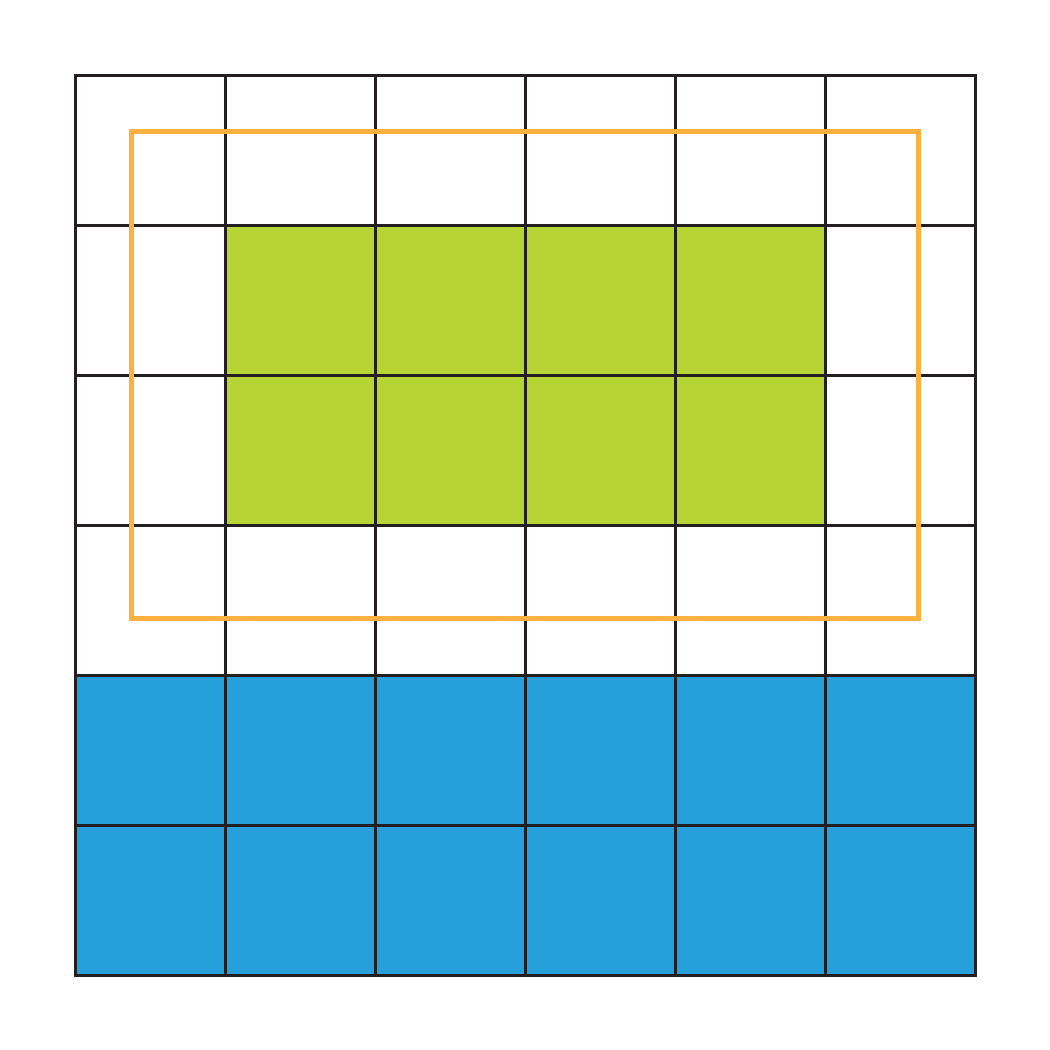
\includegraphics[width=\textwidth]{images/classification_sv}
			\caption{Swept volume}
			\label{fig:classification_sv}
		\end{subfigure}\\
		\begin{subfigure}[t]{0.3\textwidth}
			\centering
			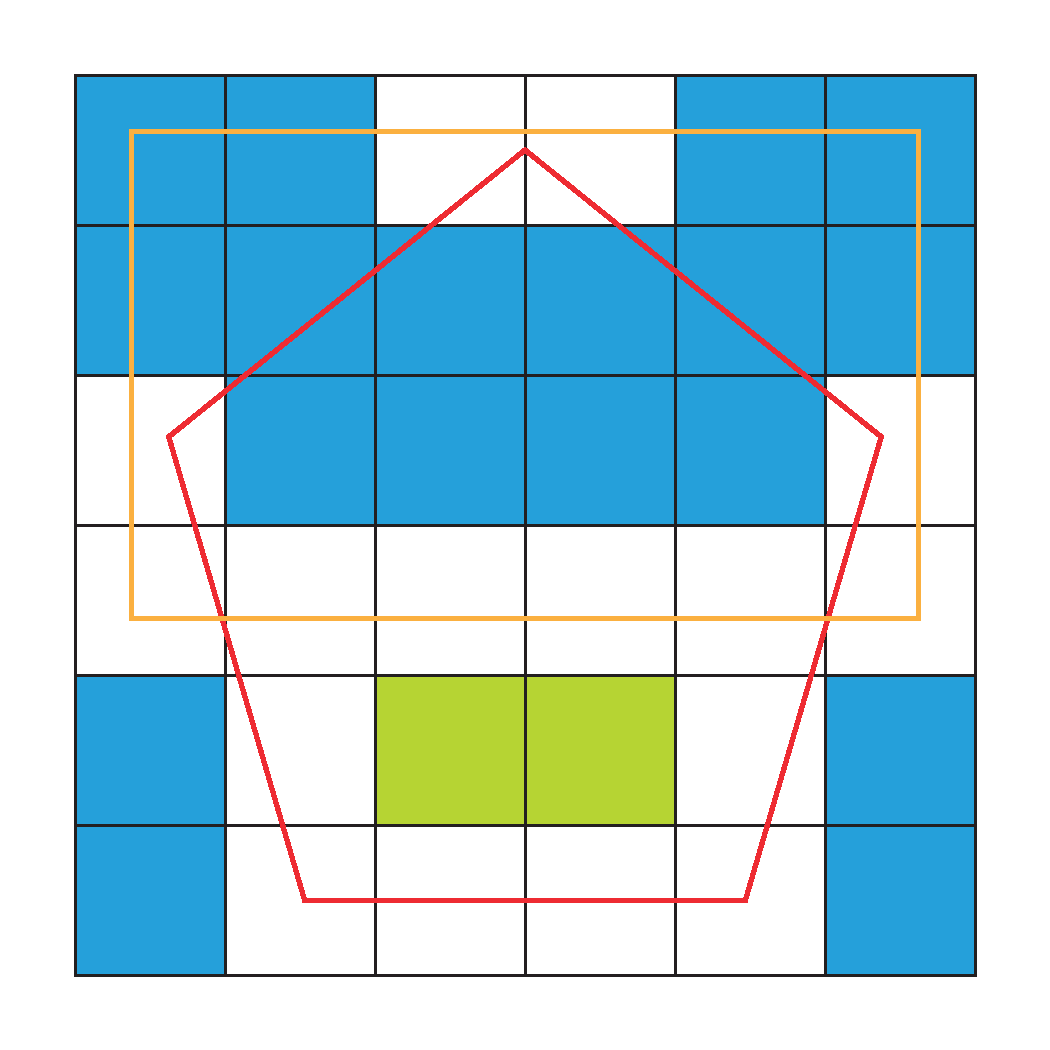
\includegraphics[width=\textwidth]{images/classification_after}
			\caption{Stock and swept volume}
			\label{fig:classification_after}
		\end{subfigure}&
		\begin{subfigure}[t]{0.3\textwidth}
			\centering
			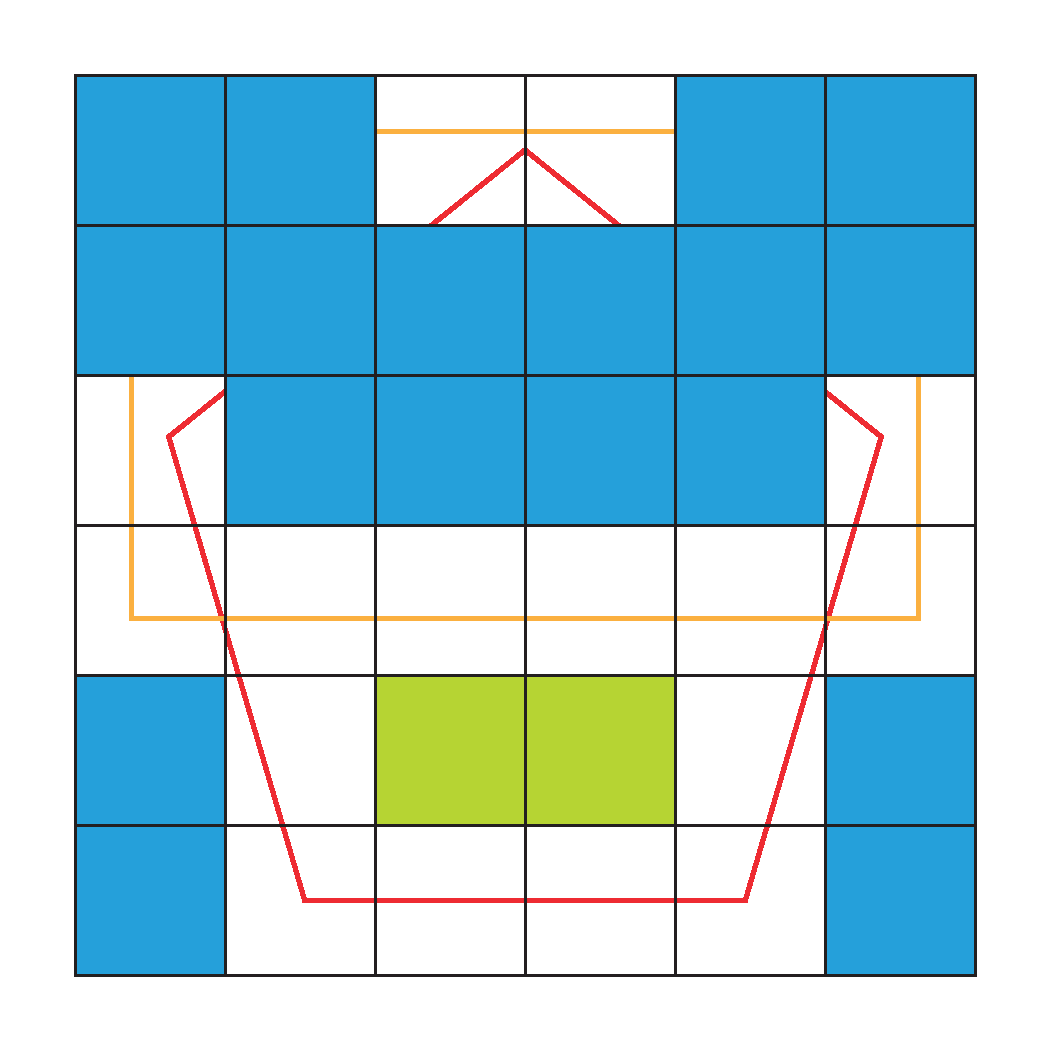
\includegraphics[width=\textwidth]{images/classification_after_removal}
			\caption{Triangle elimination}
			\label{fig:classification_after_removal}
		\end{subfigure}\\
	\end{tabular}
	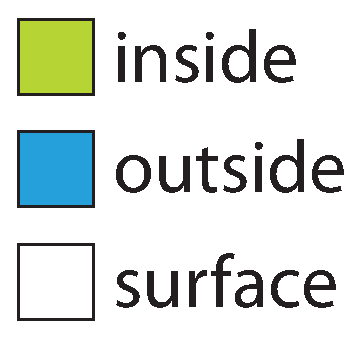
\includegraphics[width=0.1\textwidth]{images/classification_legend}
	\caption[Cell classification]{
		Principle of classifying cells according to the added mesh.
		The classification of the regular grid with a stock mesh, before a swept volume has been added, is shown in \subref{fig:classification_before}.
		The classification of the regular grid with regard to a new swept volume is shown in \subref{fig:classification_sv}.
		When the swept volume is added, both classifications are combined as shown in \subref{fig:classification_after}.
		Finally, triangles in outside cells can be removed as shown in \subref{fig:classification_after_removal}, cutting down the total number of stored triangles.
		For raycasting, only surface cells are relevant.
	}
	\label{fig:classification}
\end{figure}

When a new swept volume is added to the grid, its triangle mesh is classified itself and merged into the existing cell classification of the grid.
By limiting the modifiability of the scene to only allow subtracting swept volumes, a set of rules for merging a new mesh's classification into the grid's one can be derived and is shown in \cref{tbl:classification_rules}.

\begin{table}[h]
	\centering
	\begin{tabular}{p{2cm}p{2cm}|p{2cm}p{2cm}p{2cm}}
		                                                                &         & \multicolumn{3}{l}{Swept volume classification} \\
		                                                                &         & outside & surface & inside                      \\
		\midrule                                                                                                                    
		\multirow{3}{*}{\parbox{2cm}{Grid \\ classification \\ before}} & outside & outside & outside & outside                     \\
		                                                                & surface & surface & surface & outside                     \\
		                                                                & inside  & inside  & surface & outside                     
	\end{tabular}
	\caption{
		Classification rules when a new swept volume is added to the grid.
		On the left is the classification of a grid cell before the new volume has been added.
		On the top is the classification of a grid cell with regard to the new volume.
		The center of the table shows the outcome when these two classifications are merged.
	}
	\label{tbl:classification_rules}
\end{table}

When a new swept volume has been classified, it is merged into the grid's classification as follows:
Grid cells which are outside the added swept volume remain unchanged.
Surface cells of the added volume become surface cells except they were outside cells before.
Cells inside a swept volume always become outside cells, as they are \enquote{cut away} by the swept volume.
The result of merging a swept volume into the grid is visualized in \cref{fig:classification_after}.
After classification is complete, all triangles in outside cells can be removed, \cf \cref{fig:classification_after_removal}.

This strategy allows to keep the total number of triangles under control as the system should be able to support a large number of swept volumes, theoretically infinite if triangles are regularly eliminated.
%
However, this kind of reduction has a significant consequence.
As the contents of outside cells are simply deleted, the stored geometries are no longer closed meshes.
\Cref{fig:cylinders_classification} shows the effects of triangle elimination by example.
Surface points can still be calculated as shown by the example of the raycast used for visualization in \cref{sec:raycasting}.

\begin{figure}[!h]
	\centering
	\begin{subfigure}[b]{0.4\textwidth}
		\centering
		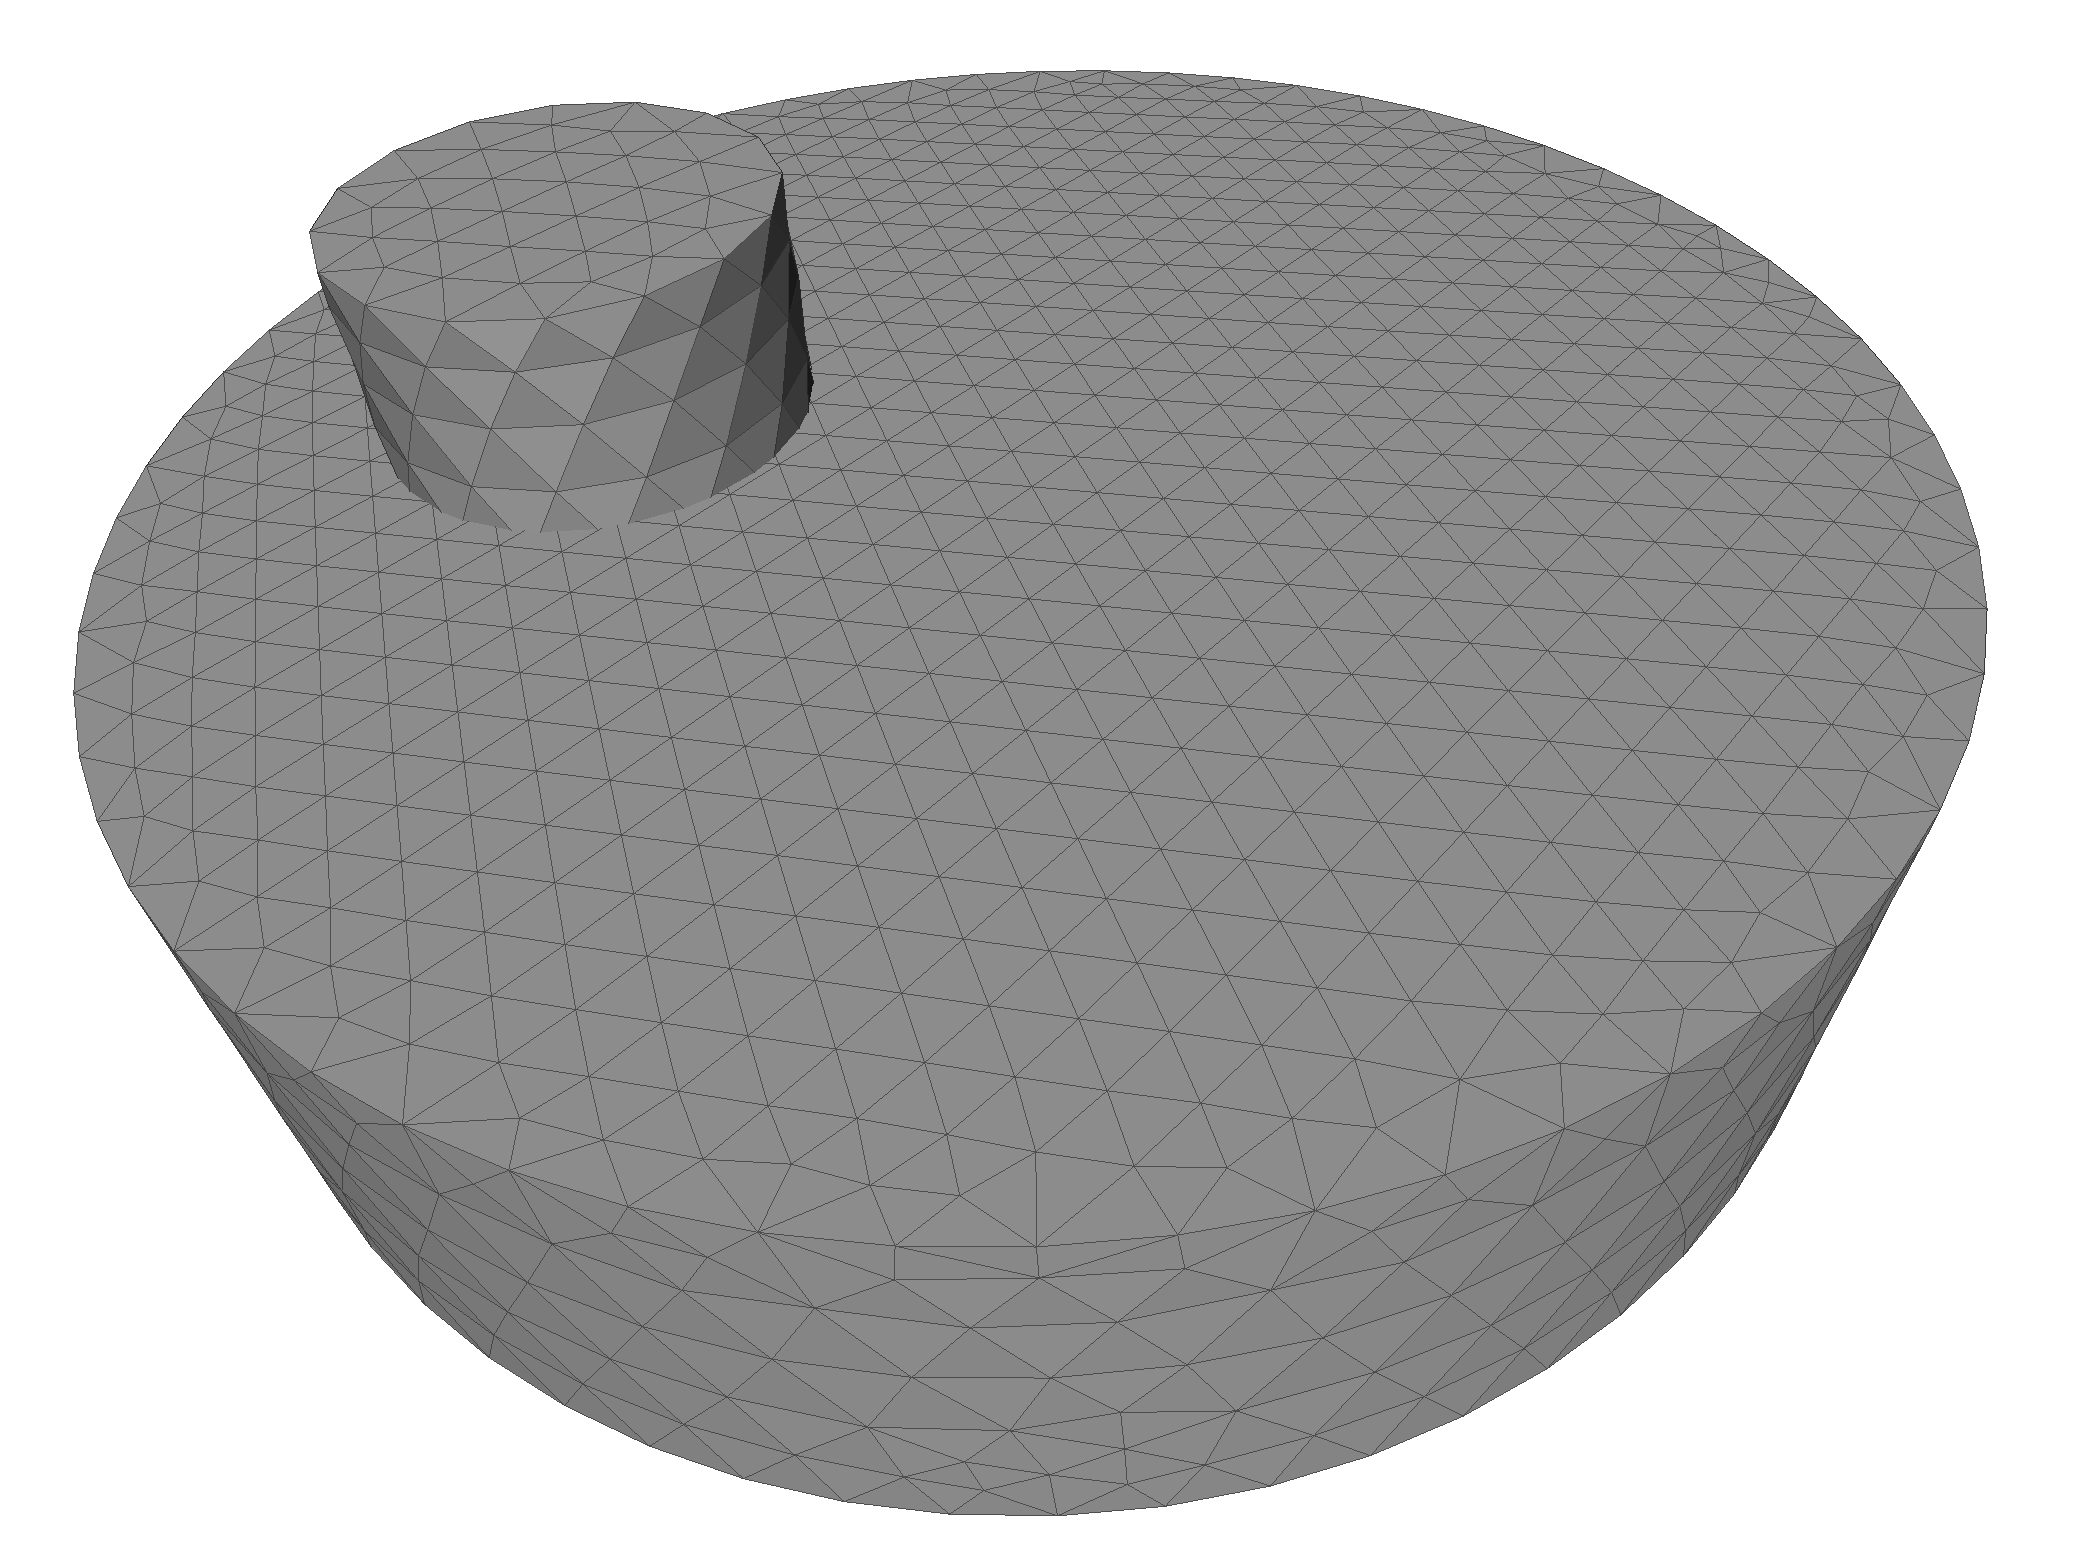
\includegraphics[width=\textwidth]{images/cylinders_classification_before}
		\caption{Before elimination.}
		\label{fig:cylinders_classification_before}
	\end{subfigure}
	\begin{subfigure}[b]{0.4\textwidth}
		\centering
		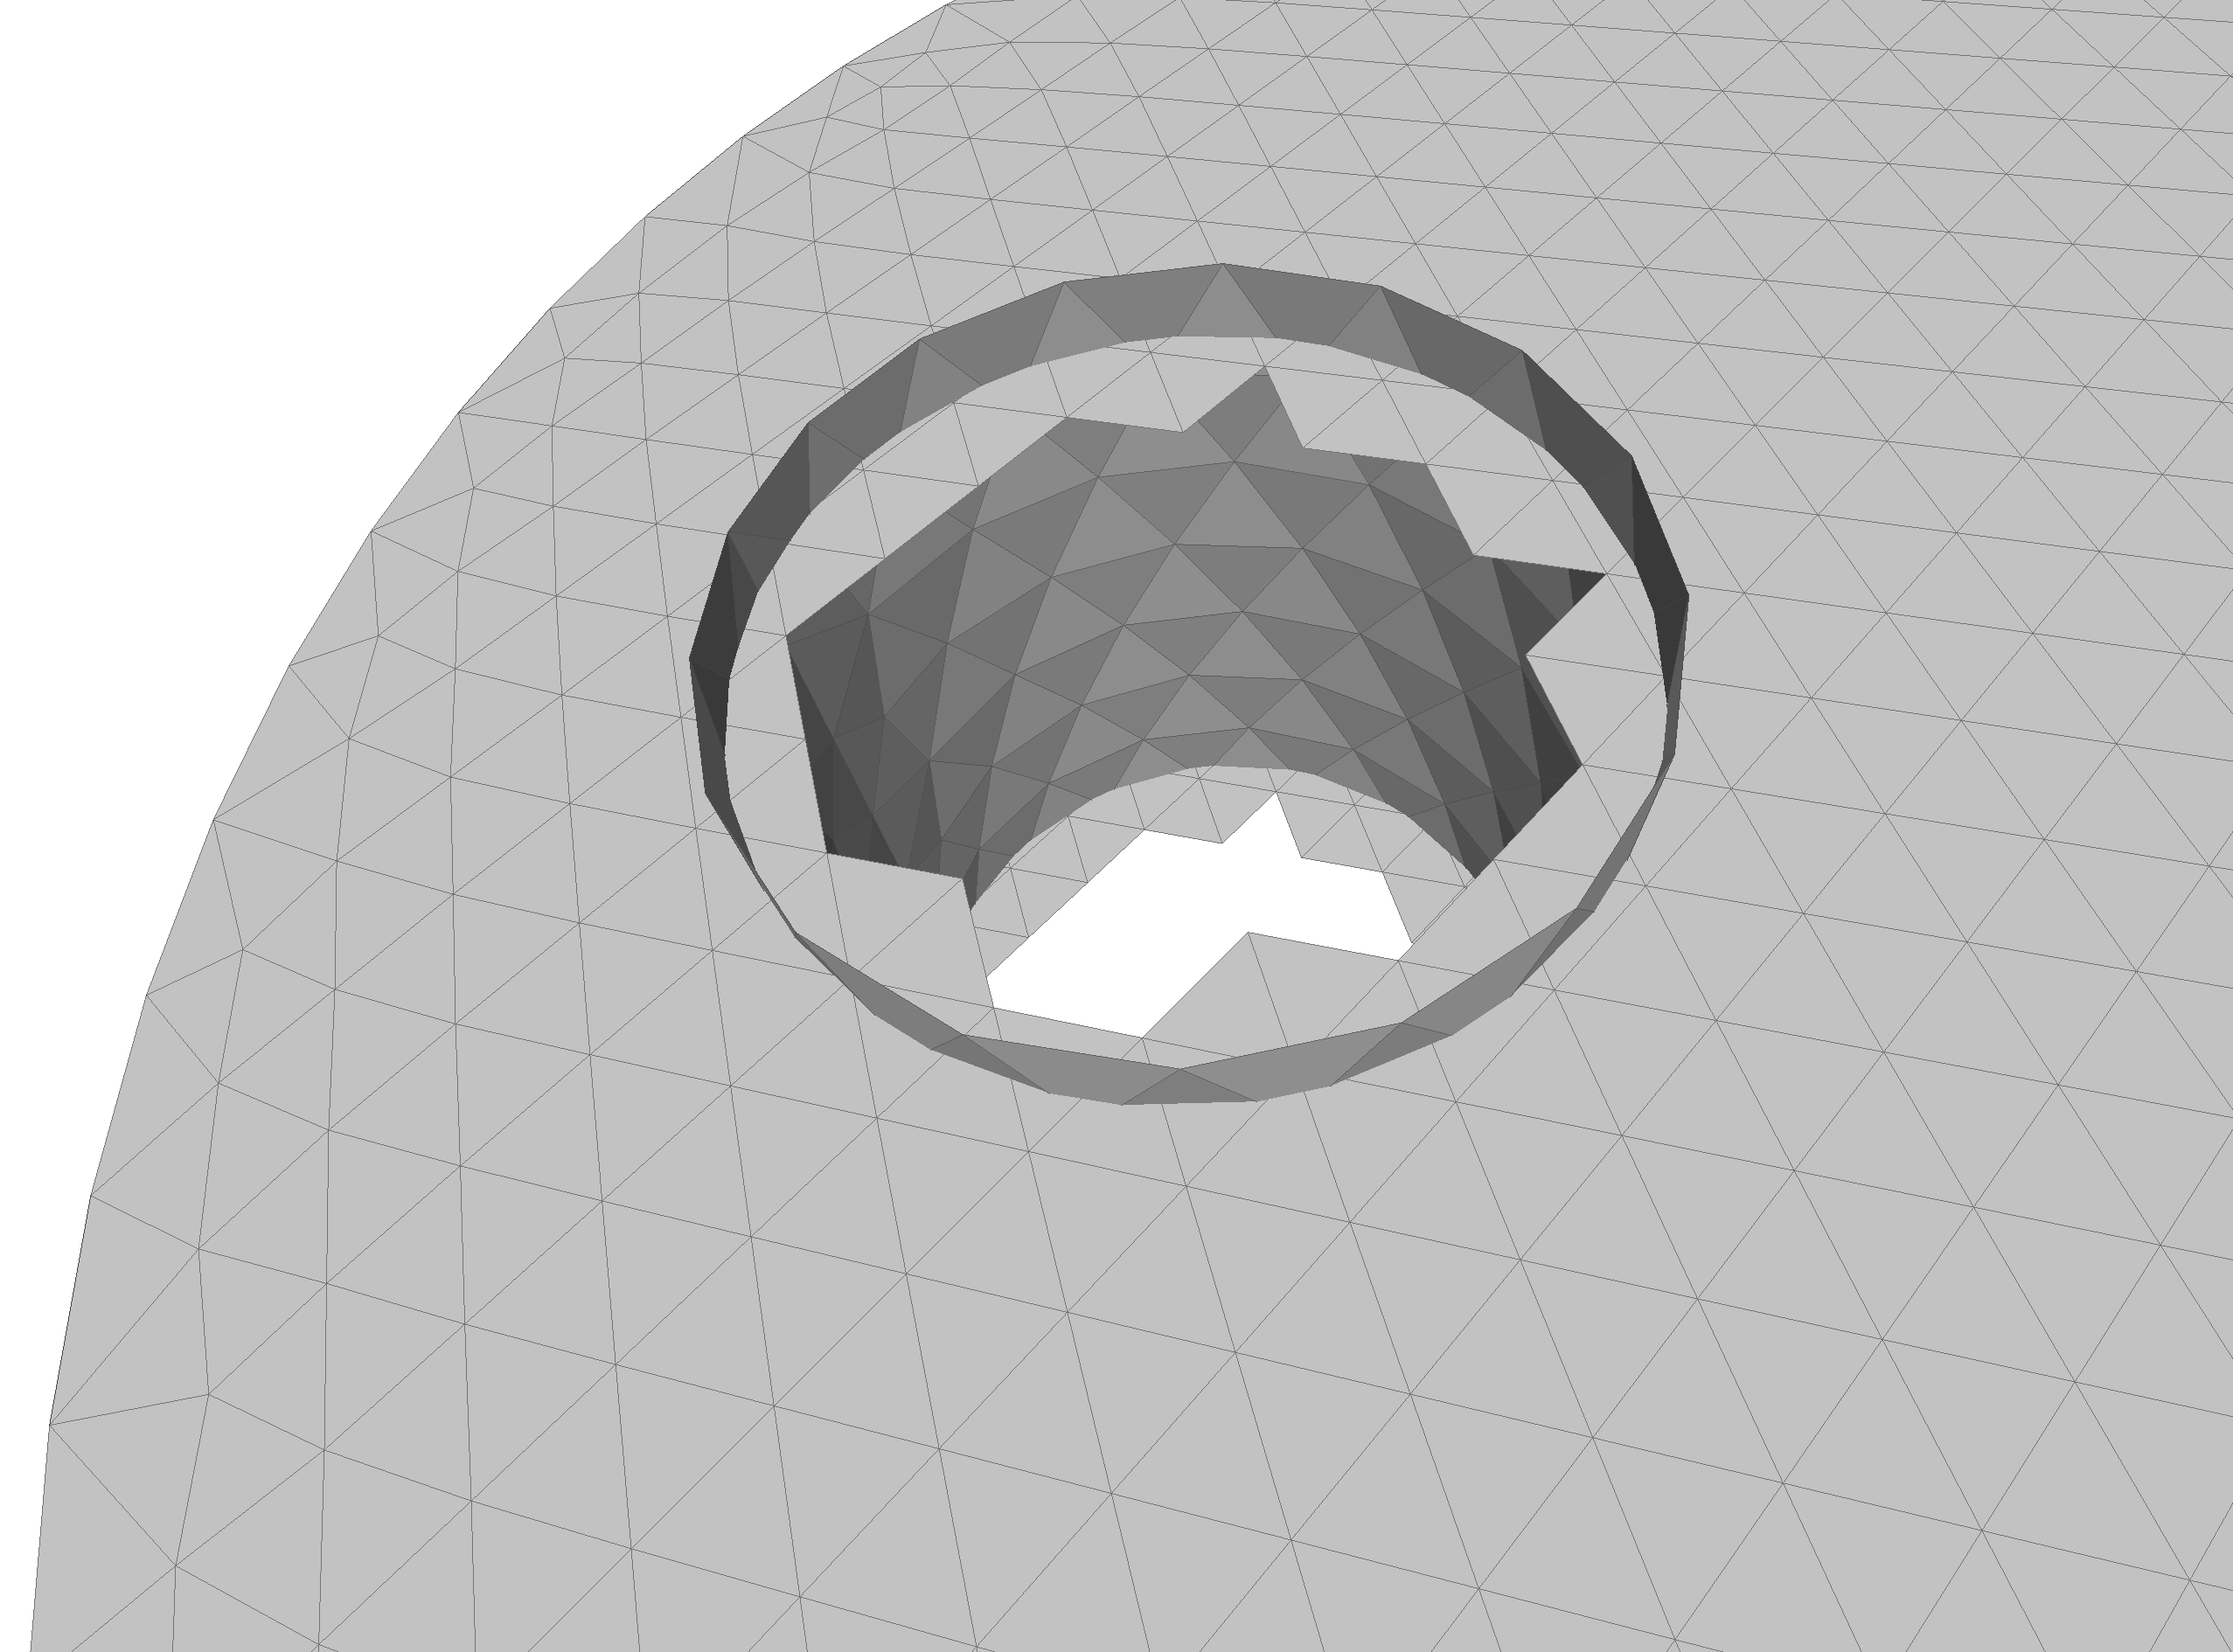
\includegraphics[width=\textwidth]{images/cylinders_classification_after}
		\caption{After elimination.}
		\label{fig:cylinders_classification_after}
	\end{subfigure}
	\caption[Triangle elimination]{
		Scene of a cylindrical stock with a smaller cylindrical swept volume.
		The left image shows both meshes before triangle elimination.
		The right image shows the resulting geometry after triangle elimination.
		Both meshes are no longer closed.
	}
	\label{fig:cylinders_classification}
\end{figure}


\subsection{Visualization by raycasting}
\label{sec:raycasting}

The VML's regular grid with its open geometries resulting from classification are visualized using an adapted raycasting approach.
For this purpose a virtual camera is placed relative to the regular grid.
The camera's position and orientation describe an image plane, \ie a rectangle, in front of the camera which will correspond to the final image.
Originating from the camera's position, a ray is sent through each pixel of the image plane into the scene.
If an intersection occurs, the pixel associated with the ray is colored according to properties of the intersected surface, \eg color, normal and material.
\Cref{fig:raycasting_principle} shows the basic principle of raycasting inside the VML.

\begin{figure}
	\centering
	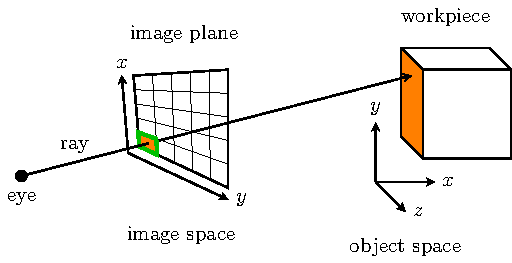
\includegraphics[width=0.7\textwidth]{raycasting}
	\caption[Raycasting principle]{
		Principle of raycasting.
		A ray is sent from an eye point, \ie camera position, through each pixel of an image plane and is traversed through the scene containing the workpiece.
		If an intersection occurs, the pixel is colored according to the intersected surface, \protect\eg color of the surface, lighting using the normal of the surface or material parameters.
		\cite{enlight_demo_workshop}.
	}
	\label{fig:raycasting_principle}
\end{figure}

When the rays hit the regular grid, they have to be traversed through the grid's cells.
A fast algorithm for traversing regular grids using a single ray is found in literature \cite{3DDDA}.
The algorithm is a slight modification of the digital differential analyzer (DDA) which is used for the rasterization of lines.
\Cref{fig:cell_traverser} shows a sketch of a single ray traversed cell by cell through the grid.
%
As neighboring rays typically take the same or a similar path through the grid, grouping rays into ray packets has been proposed as a good optimization \cite{packet_caster}.
This approach has been implemented for the VML using CPU SIMD vector extensions like SSE and AVX  \cite{enlight} and the Intel Xeon Phi many-core architecture.
\Cref{fig:slice_traverser} shows a sketch of a ray packet traversed slice by slice through the grid.

\begin{figure}
	\centering
	\begin{subfigure}[t]{0.44\textwidth}
		\centering
		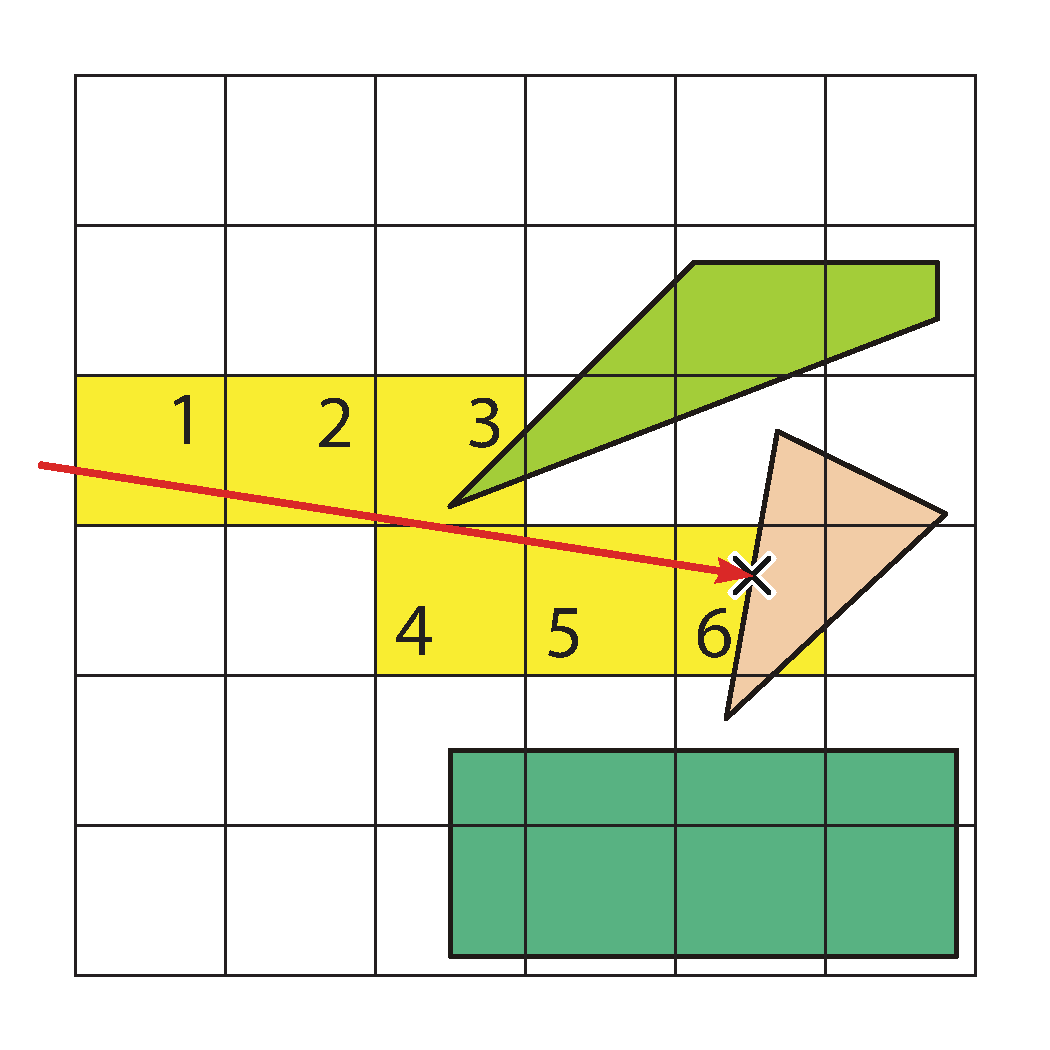
\includegraphics[width=\textwidth]{images/cell_traverser}
		\caption{Single ray.}
		\label{fig:cell_traverser}
	\end{subfigure}
	\begin{subfigure}[t]{0.44\textwidth}
		\centering
		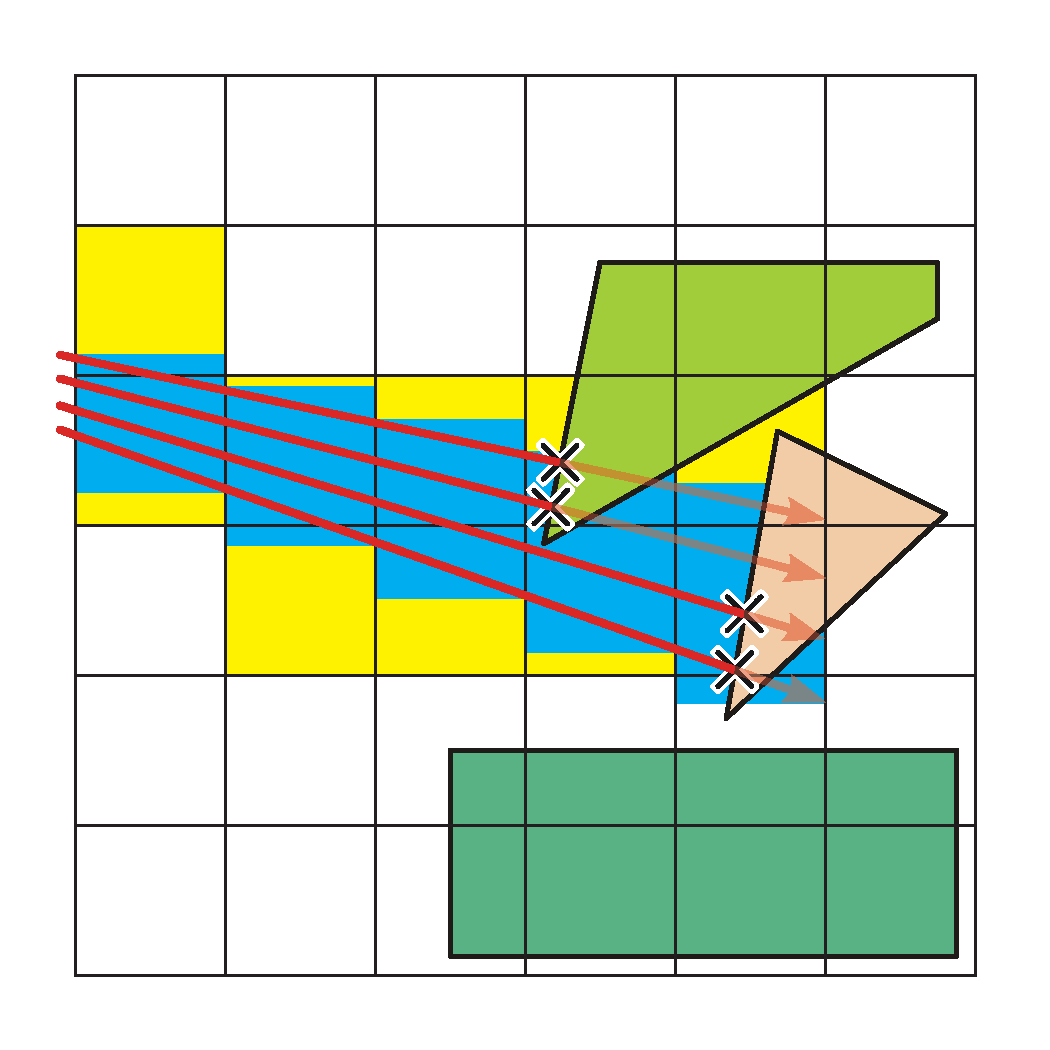
\includegraphics[width=\textwidth]{images/slice_traverser}
		\caption{Ray packet.}
		\label{fig:slice_traverser}
	\end{subfigure}
	\caption[Single ray and ray packet traverser]{
		Traversing a regular grid with a single ray, cell by cell, left image, and a ray packet, slice by slice, right image.
	}
	\label{fig:traverser}
\end{figure}

Cells classified as outside or inside are empty, \ie contain no triangles, but each surface cell contains triangles which can potentially intersect the ray.
A surface cell also typically contains parts, \ie meshes, of multiple swept volumes which are called structures in the context of a cell.
Upon entry into a surface cell, the ray has to determined the number of structures, \ie swept volumes, the ray's entry point is inside of.
This number is called the inside counter.
The stock volume is handled specially during the raycast, as it is inverted and turned into a swept volume itself to allow uniform handling.
After the inside counter has been determined, all intersections of the ray with structures inside the cell are iterated from the nearest to the farthest.
During this iterating the inside counter is modified on each structure entry or exit to constantly reflect the number of structures the ray is currently inside.
If the counter becomes zero, the surface has been reached and a hit is reported with data from the hit triangle which is later used to color the final image of the scene.
\Cref{fig:raycast} shows a detailed example of such an intersection procedure and explains the algorithmic steps to retrieve the surface hit.

\begin{figure}
	\centering
	\begin{subfigure}[t]{0.44\textwidth}
		\centering
		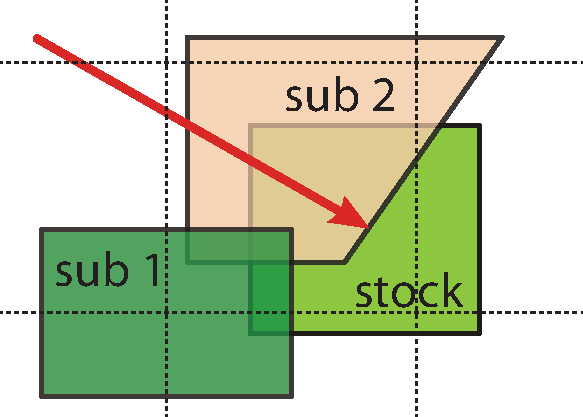
\includegraphics[width=\textwidth]{images/raycast_grid}
		\caption{Conceptual raycast.}
		\label{fig:raycast_grid}
	\end{subfigure}
	~
	\begin{subfigure}[t]{0.44\textwidth}
		\centering
		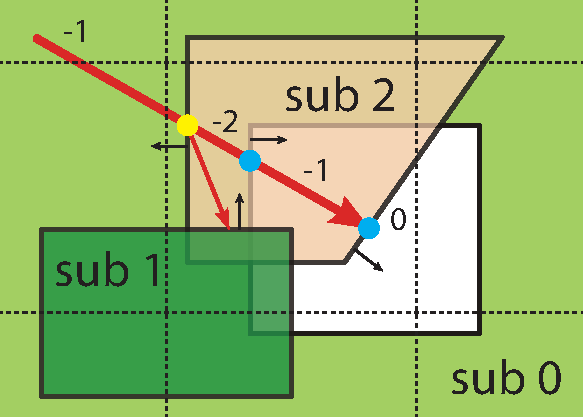
\includegraphics[width=\textwidth]{images/raycast_inside_counter}
		\caption{Implementation of raycast.}
		\label{fig:raycast_inside_counter}
	\end{subfigure}
	\caption[Raycasting interiors]{
		Interiors of the raycasting implementation.
		Upon cell entry, the inside counter is determined.
		Firstly, all intersections of the ray with structures inside the cell are calculated.
		The ray hits the structures sub 0 and sub 2.
		The surface normal of the nearest hit point with sub 2 points into a different half space than the ray direction.
		Therefore, the ray is outside sub 2 upon entry.
		The normal of the nearest hit point with sub 0 points into the same half space than the ray direction.
		Thus, the ray is inside sub 0 at the entry point.
		As the ray does not hit sub 1, a secondary ray is sent to a reference point on a triangle of sub 1.
		As the normal of sub 1 points into a different half space than the secondary ray, the ray is outside sub 1.
		Consequently, as the ray is only inside one structure, sub 0, the inside counter is initialized with -1.
		Then, all previously calculated intersections of the primary ray are ordered ascendingly by distance to the cell entry point and iterated over.
		At each intersection point, the surface normal is again compared with the ray direction.
		If they point into the same half space the structure is exited, otherwise entered.
		Entries decrease the inside counter and are marked with a yellow dot.
		Exists increase the inside counter and are marked with a blue dot.
		When the counter reaches zero, the surface point has been found.
	}
	\label{fig:raycast}
\end{figure}


\subsection{Regular grid interface}
\label{sec:vml_implementation}

To allow the extraction methods presented in this thesis to interface with the regular grid data structure, a few implementation details are needed.
This information conceptually reflects the actual implementation, providing a simplified but sufficient abstraction.

The regular grid data structure relies on a few classes shown in \cref{fig:vml_datamodel}.
The \var{RegularGrid} class basically stores a bit of meta data together with a large set of cells.
The meta data consists of the grid's axis-aligned bounding box (AABB), \var{aabb}, the size of a cell in one dimension, \var{cellSize}, as well as the number of cells in each dimension, \var{cellCount}.
The grid's cells are stored linearized in a flat array.

An axis-aligned bounding box is represented by the \var{Extends} class.
It stores two vertices, \var{lower} and \var{upper}, which contain the minimum and maximum values for each Cartesian coordinate axis.

The cells of the regular grid are modeled by the \var{Cell} class.
Each cell contains its own bounding box, \var{aabb}, the classification of the cell, \var{classification}, and an array of the triangles contained within this cell, \var{triangles}.

Each triangle, described by the class \var{Triangle}, stores its three vertices in counterclockwise order in the member \var{vertices}.
Additionally, the normal of the triangle is stored in \var{normal}, computed from the triangle's vertices for performance reasons.
Especially intersection tests, \eg during raycasting or classification, read this field very frequently and benefit from precomputation.
Each triangle also stores an unsigned integer, \var{structure}, referencing the swept volume/structure this triangle belongs to.
This field is used to group triangles inside a cell by the swept volume they originated from.

Finally, the \var{Vertex} class represents a simple 3-dimensional spatial point, storing the coordinates in its \var{values} member.

\begin{figure}
	\centering
	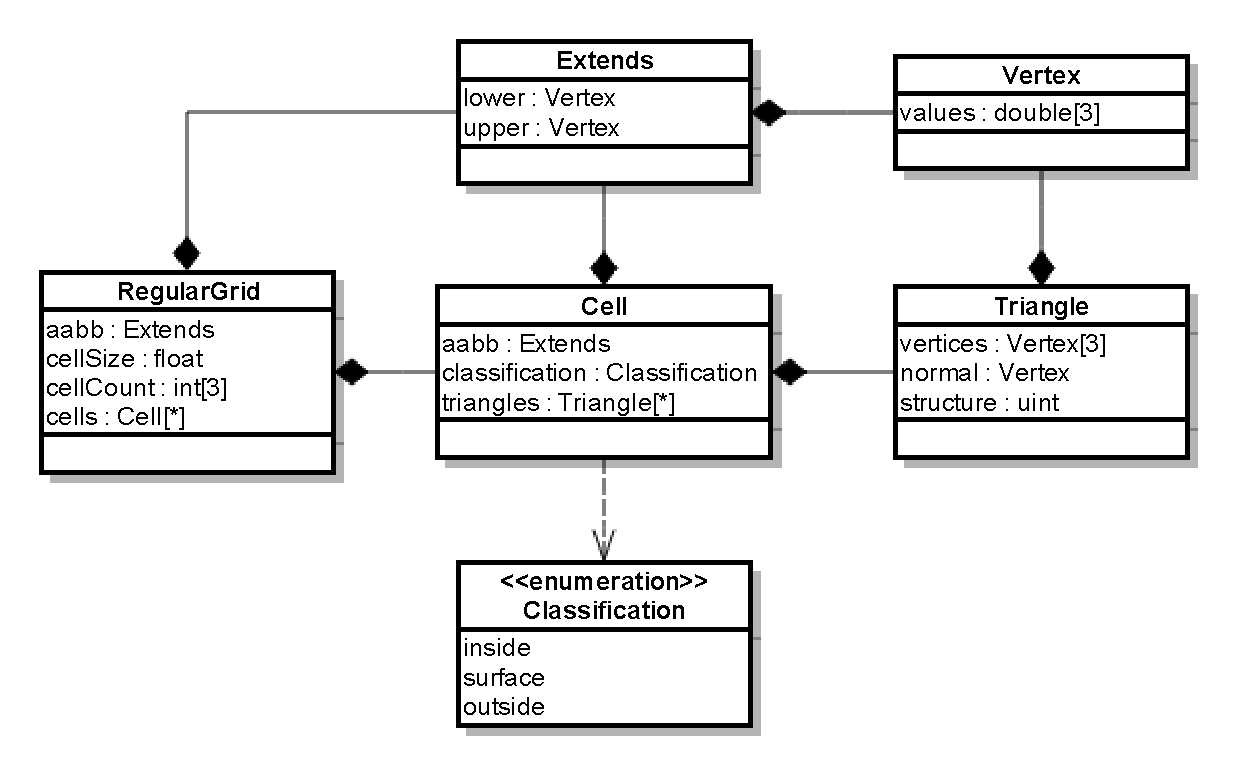
\includegraphics[width=0.9\textwidth]{vml_datamodel}
	\caption[VML UML class diagram]{
		Simplified UML class diagram of the VML data model.
	}
	\label{fig:vml_datamodel}
\end{figure}
